% Created 2024-08-11 Sun 23:47
% Intended LaTeX compiler: xelatex
\documentclass[a4paper,11pt,twoside]{article}
\usepackage{graphicx}
\usepackage{longtable}
\usepackage{wrapfig}
\usepackage{rotating}
\usepackage[normalem]{ulem}
\usepackage{amsmath}
\usepackage{amssymb}
\usepackage{capt-of}
\usepackage{hyperref}
\usepackage{libertine} \usepackage{amsmath}
\usepackage[width=200.00mm, height=240.00mm, left=3cm, right=3cm, top=3 cm, bottom=3cm]{geometry}
\usepackage{graphicx}
\graphicspath{ {./images/} }
\usepackage{multicol}
\author{Ryan P. Lynch}
\date{\today}
\title{Program 4A}
\hypersetup{
 pdfauthor={Ryan P. Lynch},
 pdftitle={Program 4A},
 pdfkeywords={},
 pdfsubject={},
 pdfcreator={Emacs 29.4 (Org mode 9.6.24)}, 
 pdflang={English}}
\usepackage{biblatex}

\begin{document}

\maketitle

\section*{Compile and Execution Linux malloc}
\label{sec:orgee21255}
\noindent
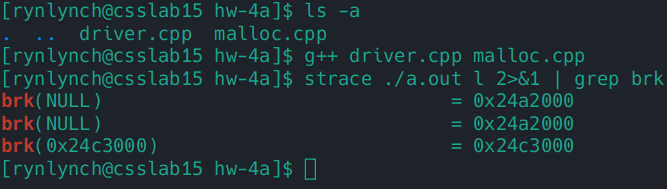
\includegraphics[width=0.5\textwidth]{linux_malloc}\\[0pt]
The screenshot above shows driver.cpp and malloc.cpp being compiled on the UW Bothell lab machine.\\[0pt]
It also shows the execution and results of the a.out binary with the 'l' switch passed to it. This result has the fewest system calls made.\\[0pt]
\section*{Compile and Execution Best Fit}
\label{sec:org0b4feeb}
\begin{multicols}{2}
\noindent
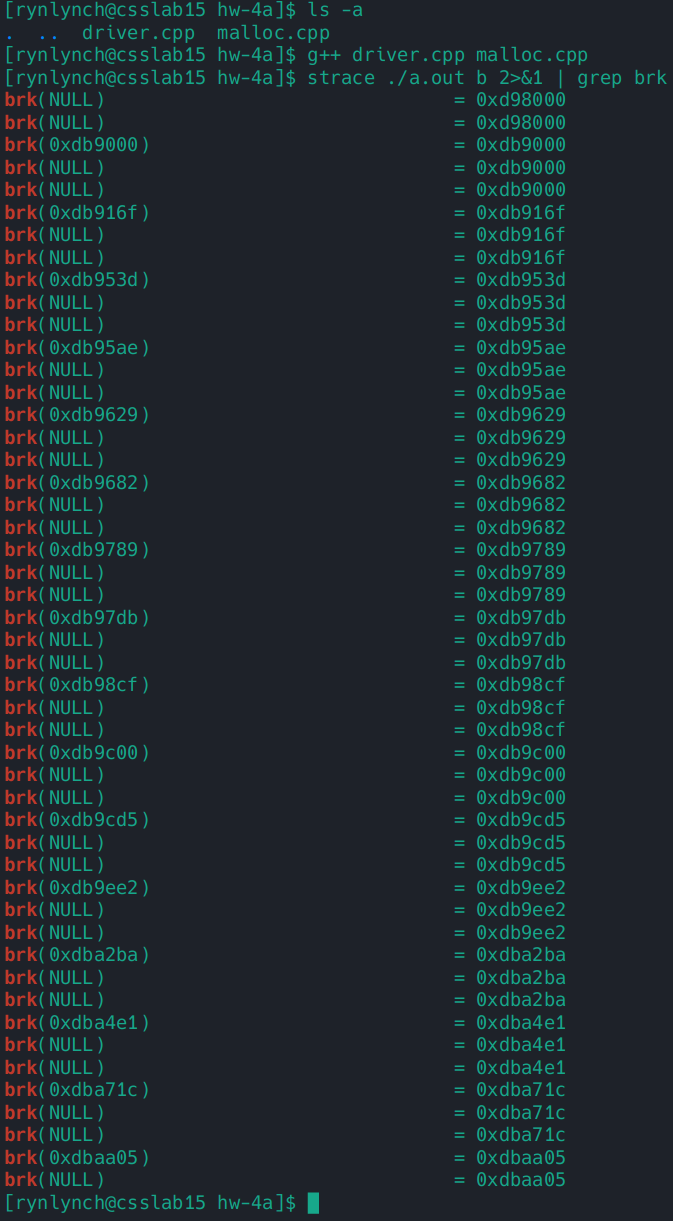
\includegraphics[width=0.5\textwidth]{ryan_b-malloc}
\noindent
The screenshot to the left shows driver.cpp and malloc.cpp being compiled on the UW Bothell lab machine.\\
\\
It also shows the execution and results of the a.out binary with the 'b' switch passed to it. Less system calls are made here than when the 'f' switch is used.\\
\end{multicols}
\section*{Compile and Execution First Fit}
\label{sec:org042a45f}
\begin{multicols}{2}
\noindent
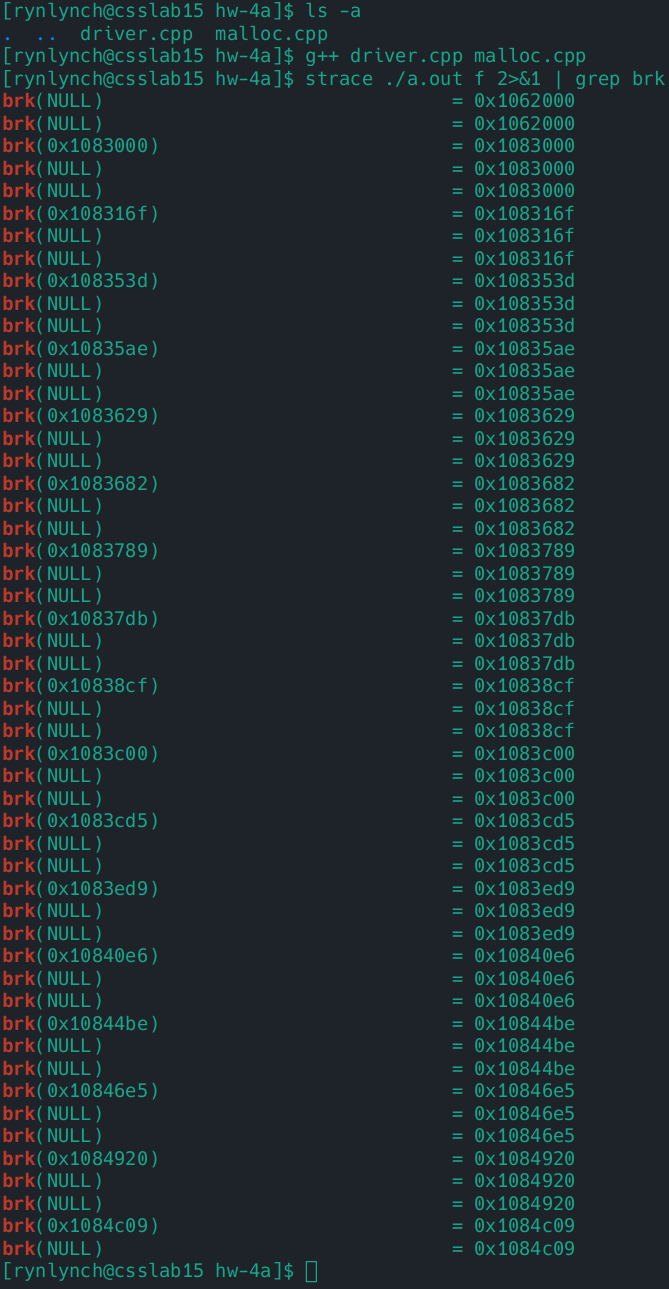
\includegraphics[width=0.5\textwidth]{ryan_f-malloc}
\noindent
The screenshot to the left shows driver.cpp and malloc.cpp being compiled on the UW Bothell lab machine.\\
\\
It also shows the execution and results of the a.out binary with the 'f' switch passed to it. More system calls are made here than when the 'b' switch is used.\\
\end{multicols}
\end{document}
